\documentclass{beamer}

% Romanian Language support
\usepackage{ucs}
\usepackage[utf8x]{inputenc}
\PrerenderUnicode{aâîțșĂÎÂȚȘ}
\usepackage[english,romanian]{babel}

\usepackage{hyperref}   % use \url{http://$URL} or \href{http://$URL}{Name}
\usepackage{verbatim}
\usepackage{underscore} % underscores need not be escaped
\usepackage{booktabs}   % nice looking tables
\usepackage{array}      % column size options in tables
\usepackage[normalem]{ulem}       % for striketrough text

\mode<presentation>
%{ \usetheme{Berlin} }

% Disable useless navigation symbols.
\setbeamertemplate{navigation symbols}{}
\setbeamertemplate{footline}[frame number]

\title[De ce asm?]{De ce să știi limbaj de asamblare?}
\institute{Informatica la Castel 2016 (Macea, Arad)}
\author[Răzvan Deaconescu]{Răzvan Deaconescu \\
razvan.deaconescu@cs.pub.ro}
\date{24 august 2016}

\begin{document}

\frame{\titlepage}

\begin{frame}{Exemplu de atac de securitate}
  \begin{itemize}
    \item TODO
  \end{itemize}
\end{frame}

\begin{frame}{Nevoia de optimizare}
  \begin{itemize}
    \item TODO
  \end{itemize}
\end{frame}

\begin{frame}{Implementare \texttt{memcpy}}
  \begin{itemize}
    \item TODO
  \end{itemize}
\end{frame}

\begin{frame}{Nevoia de debugging}
  \begin{itemize}
    \item TODO
  \end{itemize}
\end{frame}

\begin{frame}{Dezvoltare low-level}
  \begin{itemize}
    \pause \item sisteme embedded / mobile
    \pause \item Board Support Package: bootloader, kernel, drivere
    \pause \item kernel development
  \end{itemize}
\end{frame}

\begin{frame}{Înțelegerea sistemului}
  \begin{itemize}
    \item TODO
  \end{itemize}
\end{frame}

\begin{frame}{John ``maddog'' Hall: The Third Language}
  \begin{itemize}
    \item \url{https://www.lpi.org/the-third-language/}
    \item \url{http://www.techworld.com/operating-systems/john-maddog-hall-why-raspberry-pi-is-only-beginning-3453073/2/}
  \end{itemize}
\end{frame}

\begin{frame}{Joel Spolsky: Law of Leaky Abstractions}
  \begin{itemize}
    \item \url{http://www.joelonsoftware.com/articles/LeakyAbstractions.html}
  \end{itemize}
\end{frame}

\begin{frame}{Parcurgerea unei matrice}
  \begin{itemize}
    \item TODO
  \end{itemize}
\end{frame}

\begin{frame}{Shlemiel the Painter's Algorithm}
  \begin{itemize}
    \item Joel Spolsky: Back to Basics: \url{http://www.joelonsoftware.com/articles/fog0000000319.html}
  \end{itemize}
\end{frame}

\begin{frame}{Înainte de a începe}
  \begin{itemize}
    \item mai des citire decât scriere
  \end{itemize}
\end{frame}

\begin{frame}{Funcționarea unității de calcul}
  \begin{itemize}
    \item TODO
  \end{itemize}
\end{frame}

\begin{frame}{Compiler Explorer}
  \begin{itemize}
    \item \url{https://gcc.godbolt.org/}
  \end{itemize}
\end{frame}

%\begin{frame}{Experimentul cu maimuțele}
%  \begin{figure}
%    \centering
%    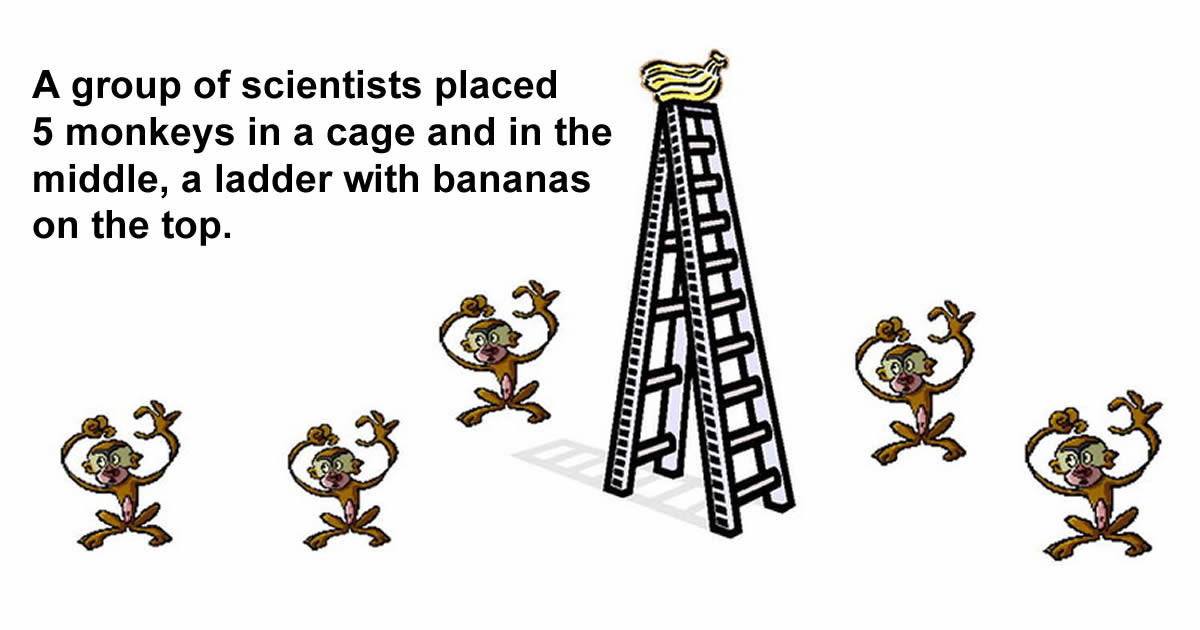
\includegraphics[width=0.8\textwidth]{img/monkey-experiment}
%  \end{figure}
%  \begin{center}
%    \tiny
%    \url{http://9gag.com/gag/aA1Z16o/curious-monkey-experiment-are-you-a-blind-follower}
%  \end{center}
%\end{frame}

%\begin{frame}{It's all about the money}
%  \begin{itemize}
%    \pause \item Ești manager.
%    \pause \item Ai nevoie ca echipa pe care o conduci să vină cu soluții creative la o problemă.
%    \pause \item Le spui că le acorzi un bonus de 25\% dacă vin astfel de soluții.
%  \end{itemize}
%  \pause
%  \begin{center}
%    Dan Pink: The Suprising Truth About What Motivates Us\\
%    \vspace{3mm}
%    \scriptsize
%    \url{http://www.ted.com/talks/dan_pink_on_motivation?language=en}
%  \end{center}
%\end{frame}

\begin{frame}{De ce e mai ușor?}
  \begin{itemize}
    \item mașini virtuale
    \item emulatoare
    \item documentație
  \end{itemize}
\end{frame}

\begin{frame}{Cum învăț/cum aprofundez}
  \begin{itemize}
    \pause \item Nu învăța ceva ca să înveți ceva / că e bine / că se caută / că vrei să știi.
    \pause \item Pune-ți obiective și învață ca o consecință. \textit{Means to an end}.
    \item competiții de tip CTF (Capture the Flag)
    \item site-uri de tip wargames
    \item profiling la aplicații de tip
    \item programează pe platforme ARM (sau MIPS): Raspberry Pi
  \end{itemize}
\end{frame}

\end{document}
